\documentclass[12pt, letterpaper]{article}
\usepackage[margin=2.5cm]{geometry}
\usepackage{times}
\usepackage{graphicx}
\usepackage[utf8]{inputenc}
\usepackage[T1]{fontenc}
\usepackage{lmodern}
\usepackage[table,xcdraw]{xcolor}
%%%%%%%%%%%%%%%%%%%%%%%%%%%%%%%%%%%%%%%%%%%%%%%%%%%%
\begin{document}
% title
\fontfamily{ptm}
\title{ENSC 351 - Lab 3: MapReduce\\ \large{- Lab Report -}}
\date{October 17, 2018}
\author{Galen Elfert, Nic Klaassen, Diane Wolf}
\maketitle
% text
\section{Explanation of workload}
	The workload invented to fit the MapReduce framework better than word counts was {[matrix multiplication | distributed sort problem | merge sort problem]...}
\subsection{Conception}
	{[Matrix multiplication | distributed sort problem | merge sort problem]} was chosen as a better alternative to word counts because...
\subsection{Speed: Single-threaded implementation}
	
\subsection{Speed: MapReduce implementation}
\subsection{Comparison}
\section{Word count efficiency}
	Both implementations of the program counted the instances of unique words (including capitalization and adjacent punctuation marks) in fifty paragraphs of Lorem Ipsum, which is 2261 words in length. They were run on the same machine with hardware to support twelve threads. Ten executions of each following implementations were conducted, with the duration and CPU usage measured with the built-in Linux \texttt{time} command:
	\begin{itemize}
	\item{single-threaded}
	\item{MapReduce, 4 threads}
	\item{MapReduce, 12 threads}
	\end{itemize}
	Additionally, call graphs for the single-threaded and MapReduce implementations were generated using Valgrind's Callgrind tool and visualized using KCachegrind.
\subsection{Single-threaded implementation}
	Table 2 below shows the execution time, as well as CPU usage, for each of the ten single-threaded word count runs. The word count program ran for a mean user time of 0.0016 seconds and a mean system time of 0.0028 - almost twice as long. This indicates that a great deal more time was spent by the CPU executing calls than in the program itself, which is consistent with single-threading. Since only one thread is tasked with carrying out many instructions, more time must be spent processing.
	
	For a graphical representation of the call map for the single-threaded word count, see figure 2 at the end of this document.
% single-threaded data
	\begin{table}[h]
	\centering
	\begin{tabular}{ccccc}
	\rowcolor[HTML]{FFFFC7} 
	\multicolumn{5}{c}{\cellcolor[HTML]{FFFFC7}\textbf{Execution times for single-threaded word count}} \\
	\rowcolor[HTML]{EFEFEF} 
	run \# & user (s) & system (s) & wall (s) & CPU usage (\%) \\
	1 & 0 & 0.004 & 0 & 0 \\
	2 & 0 & 0.008 & 0.01 & 0 \\
	3 & 0.004 & 0 & 0.02 & 0 \\
	4 & 0 & 0.004 & 0.01 & 0 \\
	5 & 0 & 0.004 & 0.01 & 0 \\
	6 & 0.004 & 0 & 0.01 & 0 \\
	7 & 0 & 0.004 & 0.02 & 0 \\
	8 & 0.004 & 0 & 0.01 & 0 \\
	9 & 0.004 & 0 & 0.04 & 0 \\
	10 & 0 & 0.004 & 0.01 & 0 \\
	\rowcolor[HTML]{D0F0D0} 
	\multicolumn{1}{r}{\cellcolor[HTML]{9AFF99}mean (s)} & 0.0016 & 0.0028 & 0.0140 & 0 \\
	\rowcolor[HTML]{ECF4FF} 
	\multicolumn{1}{r}{\cellcolor[HTML]{DAE8FC}std. dev. (s)} & 0.0021 & 0.0027 & 0.0107 & 0
	\end{tabular}
	\caption{Duration of single-threaded implementation measured by \texttt{time}}
	\end{table}
\subsection{MapReduce implementation}
	The MapReduce implementation of the word count was tested with four threads and then the full twelve threads the machine was capable of supporting. Tables 3 and 4 below show the execution time, as well as CPU usage, for each of the ten word counts run with MapReduce with four and twelve threads, respectively. Note that the greater the quantity of threads used to multithread, the slower the program execution becomes. Further, as the thread count increased, the CPU usage also appeared to increase, going from an average of 10\% with four threads to an average of 40\% with 12 threads.

	The four- and twelve-threaded MapReduce implementation timings both showed a greater user time compared to system time, on average. With four threads, the mean user time was 0.0084 seconds and the mean system time was 0 seconds. With twelve threads, the mean user time was 0.0104 seconds and the mean system time was 0.0040 seconds. This meant most of the time was spent in the program, not the CPU as was the case with single-threading.

	For a graphical representation of the call map for the MapReduce word count, see figure 3 at the end of this document.
\newpage
% MapReduce data (4 threads)
	\begin{table}[h]
	\centering
	\begin{tabular}{ccccc}
	\multicolumn{5}{c}{\cellcolor[HTML]{FFFFC7}\textbf{Execution times for MapReduce word count - 4 threads}} \\
	\cellcolor[HTML]{EFEFEF}run \# & \cellcolor[HTML]{EFEFEF}user (s) & \cellcolor[HTML]{EFEFEF}system (s) & 				\cellcolor[HTML]{EFEFEF}wall (s) & \cellcolor[HTML]{EFEFEF}CPU usage (\%) \\
	1 & 0.008 & 0 & 0.02 & 0 \\
	2 & 0.008 & 0 & 0.03 & 0 \\
	3 & 0.008 & 0 & 0.02 & 0 \\
	4 & 0.008 & 0 & 0.02 & 0 \\
	5 & 0.008 & 0 & 0.01 & 0 \\
	6 & 0.008 & 0 & 0.02 & 0 \\
	7 & 0.008 & 0 & 0.01 & 0 \\
	8 & 0.008 & 0 & 0.02 & 0 \\
	9 & 0.008 & 0 & 0.03 & 0 \\
	10 & 0.012 & 0 & 0.01 & 100 \\
	\rowcolor[HTML]{D0F0D0} 
	\multicolumn{1}{r}{\cellcolor[HTML]{9AFF99}mean (s)} & 0.0084 & 0 & 0.0190 & 10.0000 \\
	\rowcolor[HTML]{ECF4FF} 
	\multicolumn{1}{r}{\cellcolor[HTML]{DAE8FC}std. dev. (s)} & 0.0013 & 0 & 0.0074 & 31.6228
	\end{tabular}
	\caption{Duration of MapReduce implementation measured by \texttt{time}, with four threads}
	\end{table}
% MapReduce data (12 threads)
	\begin{table}[h]
	\centering
	\begin{tabular}{ccccc}
	\multicolumn{5}{c}{\cellcolor[HTML]{FFFFC7}\textbf{Execution times for MapReduce word count - 12 threads}} \\
	\rowcolor[HTML]{EFEFEF} 
	run \# & user (s) & system (s) & wall (s) & CPU usage (\%) \\
	1 & 0.008 & 0.004 & 0.01 & 0 \\
	2 & 0.008 & 0.008 & 0.03 & 0 \\
	3 & 0.008 & 0.008 & 0.01 & 0 \\
	4 & 0.008 & 0.004 & 0.01 & 0 \\
	5 & 0.016 & 0 & 0.01 & 100 \\
	6 & 0.008 & 0.004 & 0.01 & 0 \\
	7 & 0.012 & 0.004 & 0.01 & 100 \\
	8 & 0.008 & 0.008 & 0.01 & 0 \\
	9 & 0.012 & 0 & 0.01 & 100 \\
	10 & 0.016 & 0 & 0.01 & 100 \\
	\rowcolor[HTML]{D0F0D0} 
	\multicolumn{1}{r}{\cellcolor[HTML]{9AFF99}mean (s)} & 0.0104 & 0.0040 & 0.0120 & 40.0000 \\
	\rowcolor[HTML]{ECF4FF} 
	\multicolumn{1}{r}{\cellcolor[HTML]{DAE8FC}std. dev. (s)} & 0.0034 & 0.0033 & 0.0063 & 51.6398
	\end{tabular}
	\caption{Duration of MapReduce implementation measured by \texttt{time}, with twelve threads}
	\end{table}
\subsection{Comparison}
	An increase in threads used in the implementation of word counts appears to correspond with a decrease in time spent performing CPU calls and an increase in time spent in the program itself. As for wall time, there was not a clear difference between implementations - the single-threaded implementation came in with a mean wall time of 0.0140 seconds, the four-threaded MapReduce implementation with a mean wall time of 0.0190 seconds, and the twelve-threaded MapReduce implementation with a mean wall time of 0.0120 seconds.
\section{Most appropriate workload for MapReduce}
	Data that needs sorting?
\section{Impact of using multiple machines on execution speed}
	
% figures
\newpage
	\begin{figure}[h]
	\centering
	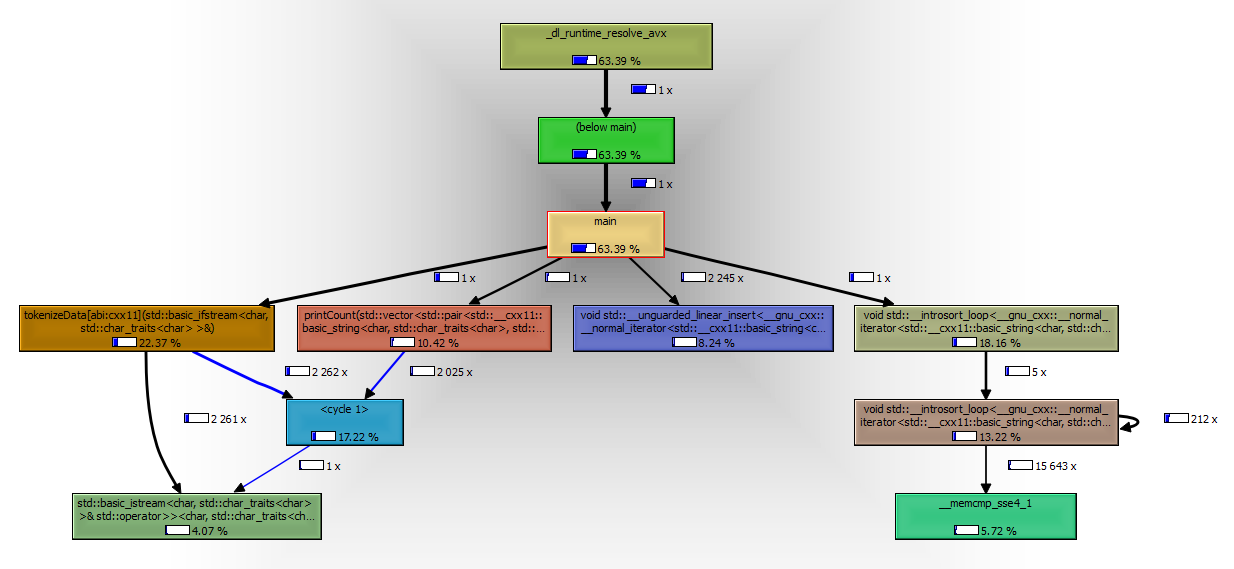
\includegraphics[width=1.35\textwidth, angle=90]{call-graph-part3-cropped}
	\caption{Call map for single-threaded implementation of word count}
	\end{figure}
\newpage
	\begin{figure}[h]
	\centering
	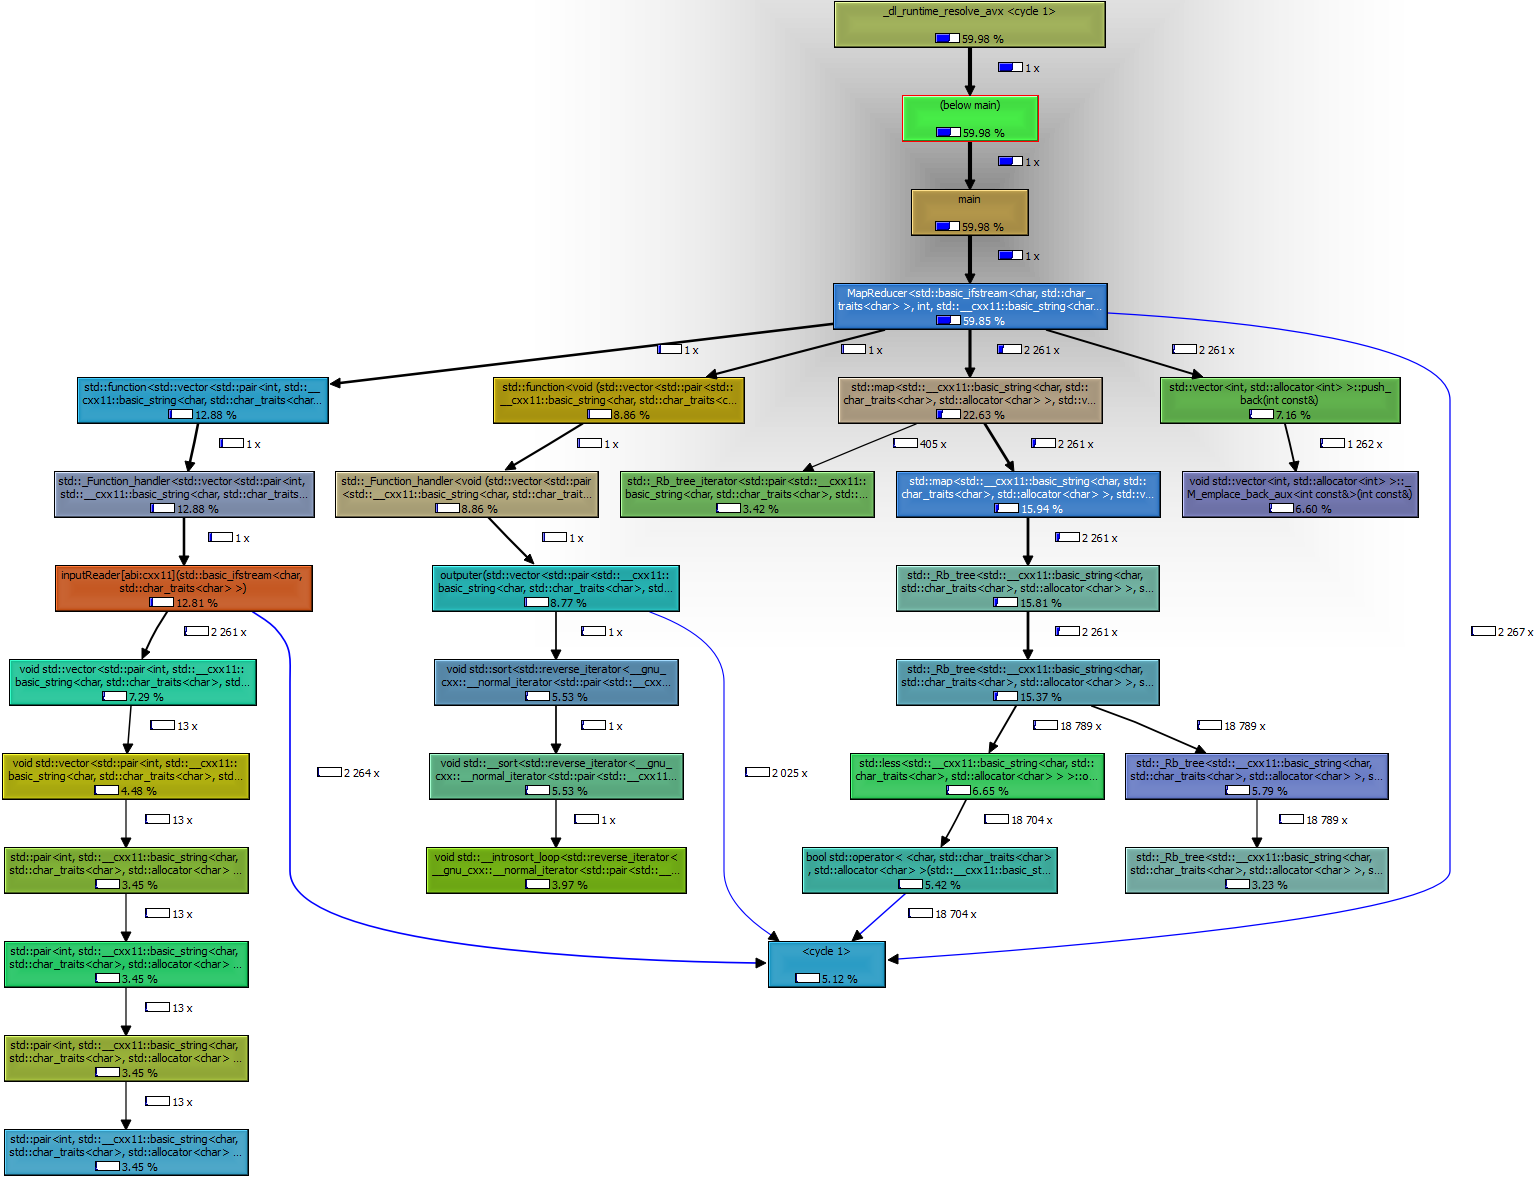
\includegraphics[width=1.35\textwidth, angle=90]{call-graph-part4-cropped}
	\caption{Call map for MapReduce implementation of word count (twelve threads)}
	\end{figure}
\end{document}